\chapter{Einleitung}\label{kap1}
\section{Motivation und Ziele der Arbeit}
Dass elektrifizierte Antriebssysteme auf lange Sicht stark an Bedeutung gewinnen werden, steht für die Akteure der Automobilbranche außer Frage. Doch obwohl Elektroautos schon seit Jahren auf dem Markt vertreten sind, bleibt die Nachfrage gering. Besonders bezüglich der Aspekte Kosten und Reichweite bestehen noch große Einschränkungen, die die Akzeptanz und Verbreitung einschränken, obwohl seitens Politik und Industrie immer weiter in die Elektromobilität investiert wird. Um die Defizite der E-Mobilität zu beheben wird seit Jahren ausgiebig an der Effizienz und den Kosten von elektrischen Automobilen geforscht und gearbeitet.
Auch das Institut für Mechatronische Systeme im Maschinenbau (IMS) der TU Darmstadt nimmt sich dieser Aufgabe an und arbeitet im Rahmen des Projektes Speed4E (Nachfolgerprojekt von Speed2E), das einen elektrifizierten Antriebsstrang mit Peak-Antriebsdrehzahlen von bis zu \SI{50 000}{min^{-1}} zum Ziel hat, an einem innovativem Schaltaktor. Das Projekt testete dabei einen neuartigen Antriebsstrang, bestehend aus zwei elektrischen Antriebseinheiten, deren Leistung sich über zwei parallelen Teilgetriebe, von denen eines schaltbar ist, summiert. Denn nicht nur in konventionellen Antrieben, sondern auch in elektrifizierten und hybriden Antrieben optimieren schaltbare Getriebe und die damit einhergehende Einstellung der Drehzahl die Fahrleistung und die Effizienz \cite{Tsch14}.
  Im Verlauf vorheriger Arbeiten wurden bereits ein linearer Tauchspulenaktor für das Zwei-Gang-Teilgetriebe ausgelegt sowie eine Elektronik und Positionsregelung dafür entwickelt. Ein zukünftiges Ziel ist es, den entwickelten Antrieb in ein Fahrzeug zu integrieren. Mit den einzelnen Hardwarekomponenten ist das zur Zeit nicht möglich. Der benötigte Bauraum sprengt den Rahmen, auch die vielen verschiedenen Schnittstellen nach außen und die Verbindungen durch Kabel der Komponenten untereinander stellen ein großes Problem dar und lassen sich auf keinen Fall so in ein Fahrzeug implementieren.
Das Ziel dieser Arbeit ist es nun, die bisherigen Funktionen auf einen Mikrocontroller zu implementieren sowie eine eingebettete Elektronik zu entwerfen, die den Aktor zu einem Smart Actuator transformiert. Die bisher zum Steuern benötigte dSpace MicroAutobox soll im Rahmen des ADPs als Reglerelement ersetzt, und die zugehörige Elektronik auf einer Platine untergebracht werden. Die Vorteile hierbei sind die starke Bauraum- und Gewichtsreduzierung sowie verringerte Kabellängen, die geringere Komplexität für Systemintegratoren und die gesenkten Kosten. Weiterhin sind die bessere Kontrollierbarkeit und die kürzere Installationsdauer zu nennen. Das Gesamtsystem ist leichter anzusteuern und besteht nicht mehr aus mehreren einzelnen Komponenten. Ein weiteres Ziel ist das Einrichten von Schutzmechanismen und Überwachungsfunktionen für den Aktor. Fehlzustände sollen erkannt und über CAN-Kommunikation übermittelt werden, sodass das übergeordnete System entsprechend reagieren kann. Der Smart Actuator kann somit seinen Status diagnostizieren und in Echtzeit auf Störungen reagieren. 
In \autoref{fig:Ziele} ist nochmal die Gegenüberstellung von Ausgangslage und Zielsetzung des Gesamtsystems dargestellt. 
\begin{figure}[H]%
\centering
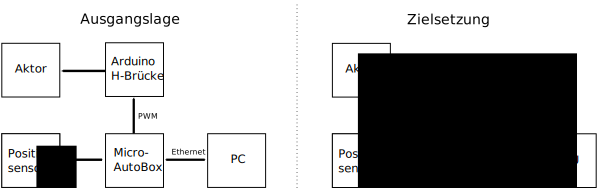
\includegraphics[width=0.9\columnwidth]{./Bilder/Ziel}%
\caption{Ausgangslage und Zielsetzung der Projektarbeit}%
\label{fig:Ziele}%
\end{figure} \indent
Auf der linken Seite sehen wir die Ausgangslage:  Die dSpace MicroAutoBox stellt dabei den Regler dar, der Istposition (bereitgestellt durch Positionssensordaten) und Sollposition (übermittelt über Ethernet vom PC) vergleicht und schließlich über pulsweitenmodulierte Spannungssignale eine H-Brücke ansteuert, welche wiederum den Aktor ansteuert. Dieser bewirkt die Bewegung der Schaltgabel und kann somit in verschiedene Gänge schalten. Auf der rechten Seite ist zu erkennen, wie das Gesamtsystem nach Abschluss der Projektarbeit optimalerweise aussehen sollte. Zentrales Element und Regler bildet hierbei die eingebettete Elektronik. Sie empfängt Daten vom Positionssensor, steuert den Aktor an und kommuniziert per CAN mit einem externen Steuergerät.

\section{Anforderungsliste}
Um das übergeordnete Ziel weiter zu spezifizieren wurde zunächst eine Anforderungsliste (\autoref{tab:Anforderungsliste}) erstellt. In dieser sind alle Forderungen an das Endprodukt gesammelt, sie dient damit als Basis und Referenz für die Produktentwicklung. Die Liste ist hierbei dynamisch, das heißt sie kann im Verlauf des Entwicklungsprozesses verändert oder ergänzt werden.  Die formulierten Anforderungen werden nach ihrer Priorität kategorisiert und einer der vier folgenden Anforderungsarten zugeordnet \cite[S.189]{2013a}. Festforderungen (FF) sind unter allen Umständen einzuhalten. Eine Erfüllung ist für eine erfolgreiche Lösung notwendig.
Bereichsforderungen (BF) geben einen Toleranzbereich an, innerhalb dessen sich der schlussendlich erreichte Wert befinden muss.
Zielforderungen (ZF) geben an, welcher Wert (auch im Hinsicht auf spätere Entwicklungen) angestrebt wird.
Wünsche (W) sollten nach Möglichkeit erfüllt werden, sind aber keine Voraussetzung. 

\begin{table}[h]
	\centering
		\captionabove{Anforderungsliste}
		\begin{tabular}{l|p{7cm}|p{7cm}}
			\textbf{Relevanz} & \textbf{Anforderung} & \textbf{Erläuterung} \\ \hline
			& &\\
			FF & Benutzerfreundliche Kommunikation durch CAN Schnittstelle & Empfang von Befehlen, Senden von Statusmeldungen \\ \hline
			FF & Nichtflüchtige Kalibrierung & Eine Kalibrierung ist nur einmalig und zur Rekalibrierung notwendig \\ \hline
			BF & Schaltzeit & < \SI{100}{ms} (Latenz zwischen Senden des Befehls und vollständig ausgeführtem Gangwechsel) \\ \hline
			FF & Selbstständige Fehlererkennung & Überstrom, Temperatur, Eingangsspannungsbereich, Dekalibrierung \\ \hline
			FF & Schnittstellen & CAN, \SI{8-16}{VDC} Versorgung, Programmierschnittstelle (für Updates \& Bugfixes) \\ \hline
			W & Wartbarkeit & Sicherung wechseln im eingebauten Zustand \\ \hline
			BF & kompakte Baugröße & 88,8x\SI{50}{mm}\\ \hline
			BF & Effizienz (gemittelt über einen Schaltvorgang) & elektrischer Wirkungsgrad > 90 \% \\ \hline
			FF & Temperaturbeständigkeit & bis \SI{105}{^\circ C} \\ \hline
			BF & Aktorüberschwingen & Toleriert, solange kein unbeabsichtigter Gangwechsel $\rightarrow$ \SI{<1}{mm} \\ \hline
			W & Schaltgabelkraft am Anschlag & möglichst gering \\ \hline
			FF & Standby & Standbyleistungsaufnahme < \SI{2}{W} \\ \hline
		\end{tabular}
	
	\label{tab:Anforderungsliste}
\end{table}

\section{Aufbau der Arbeit}
Nachdem in der Anforderungsliste nach \autoref{tab:Anforderungsliste} die Ziele der vorliegenden Arbeit definiert wurden, soll nun das weitere Vorgehen zum Erreichen der Zielsetzung erläutert werden. Zunächst werden in \autoref{kap2} der Stand des Prüfstands vor Beginn des Projektes sowie wichtige Grundlagen als Basis für die weitere Bearbeitung und zum besseren Verständnis dargelegt. \autoref{kap3} stellt das allgemeine methodische Vorgehen der Arbeit vor und erklärt die Entwicklungsmodelle und Testkonzepte, die angewendet wurden.
In \autoref{ch:komp} werden die verschiedenen Komponenten, die für die Elektronik benötigt werden, und ihre Funktionen beschrieben.  
In \autoref{kap5} soll schließlich der endgültige Platinenentwurf inklusive Methoden zur EMV-Verbesserung vorgestellt werden.
In Kapitel 6 wird nach der Vorstellung der entwickelten Software auch auf Optimierungsmöglichkeiten der Programmierung eingegangen.
Anschließend wird in \autoref{kap7} das Endprodukt auf seine Performance analysiert sowie die anfangs gestellten Anforderungen überprüft. Zum Abschluss wird in Kapitel 8 ein Fazit gezogen sowie ein Ausblick für weitere Forschungsarbeiten gegeben.